% BitCal-TTS — publication-style arXiv manuscript (target ~12 pages PDF with appendix).
% Compile: pdflatex (twice) + bibtex, or latexmk -pdf.
\documentclass[11pt]{article}

\usepackage[margin=1in]{geometry}
\usepackage[T1]{fontenc}
\usepackage[utf8]{inputenc}
\usepackage{microtype}
\usepackage{graphicx}
\usepackage{booktabs}
\usepackage{amsmath,amssymb}
\usepackage{algorithm}
\usepackage{algorithmic}
\usepackage{tikz}
\usetikzlibrary{arrows.meta,positioning,fit,calc,shapes.misc,backgrounds}
\usepackage{xcolor}
\usepackage[numbers,sort&compress]{natbib}
\usepackage{enumitem}
\usepackage{subcaption}
\usepackage{hyperref}

\hypersetup{
  colorlinks=true,
  linkcolor=blue,
  citecolor=blue,
  urlcolor=blue,
}

\setlist{nosep,leftmargin=*}

\graphicspath{{media/}}

\title{BitCal-TTS: Bit-Calibrated Test-Time Scaling for Quantized Reasoning Models}

\author{
  Sai Babu\\
  \texttt{update-email@domain.com}
}

\date{}

\begin{document}
\maketitle

\begin{abstract}
Quantization makes large reasoning models practical under tight memory budgets, but it can distort the online signals that drive adaptive test-time compute allocation. Under a fixed per-example cap on newly generated tokens, miscalibrated ``confidence'' can produce harmful early halting: the model may surface a plausible final line while still being wrong, or the policy may stop before reasoning has stabilized. We study this interaction for greedy 4-bit inference and propose \textbf{BitCal-TTS}, a lightweight runtime controller that couples (i) cheap online proxies for uncertainty and stability, (ii) a bit-conditioned confidence rescaling that is conservative at low nominal precision, and (iii) a bit-aware post-marker confirmation horizon tailored to GSM8K-style outputs. The method requires \emph{no} fine-tuning of the base model and plugs into standard Hugging Face 4-bit inference with forward hooks for logits and last-layer hidden states~\cite{transformers}.

On GSM8K~\cite{cobbe2021gsm8k} with Qwen2.5 Instruct models~\cite{qwen25technical}, BitCal-TTS improves exact-match accuracy over a non-bit-aware adaptive baseline at 7B/14B while retaining large savings versus fixed-budget decoding. At budget $B{=}512$, gains are $+3.7$ accuracy points (7B) and $+2.8$ points (14B), with premature-stop rates reduced from $14.8\%$ to $11.1\%$ (7B) and from $17.1\%$ to $11.4\%$ (14B). We release code and figure-generation scripts for full reproduction.
\end{abstract}

\noindent\textbf{Keywords:} test-time scaling, quantization, adaptive halting, GSM8K, uncertainty proxies

\section{Introduction}
Reasoning-centric language models benefit from allocating additional tokens at inference time. Chain-of-thought style deliberation and related sequential strategies can improve verifiable accuracy on math and logic tasks~\cite{wei2022cot,snell2024scalingllmtesttime,muennighoff2025s1}. In deployment, however, practitioners almost always bound generation: \texttt{max\_new\_tokens} caps latency and cost, and product surfaces often add early-exit heuristics when an answer ``looks complete''.

This paper focuses on a common production stack: a \emph{causal} instruction-tuned model served with post-training quantization (e.g., 4-bit weights via bitsandbytes~\cite{bitsandbytes,dettmers2023qlora}) under a hard token budget $B$. Quantization widens the set of models that fit consumer GPUs, but it also changes the geometry of logits and hidden states. Entropy and stability cues measured during decoding can become miscalibrated relative to full precision: the policy may \emph{appear} confident while still being unreliable, which increases the risk of stopping too soon~\cite{kadavath2022know,manakul2023selfcheckgpt}. The failure mode is not only lower final accuracy, but \emph{wasted} adaptive compute when the controller halts on a spurious ``final'' segment.

\paragraph{Contributions.}
\begin{itemize}
  \item We formalize a budgeted, stepwise inference loop for quantized causal LMs with halting actions $\{\texttt{continue},\texttt{stop},\texttt{escalate}\}$, contrasting (a) fixed decoding, (b) adaptive decoding with a precision-\emph{agnostic} calibrator, and (c) BitCal-TTS.
  \item We describe transparent, implementation-aligned proxies for entropy, textual trace stability, and hidden-state drift, and show how a bit-width multiplicative scale makes stop decisions conservative at aggressive quantization.
  \item We document a GSM8K-oriented \emph{post-marker} confirmation rule: once the standard \texttt{\#\#\#\#} answer delimiter appears, decoding switches to a bit-conditioned tail budget before termination. This differs from treating the delimiter as an immediate halt signal, which is brittle under 4-bit noise.
  \item We report GSM8K results for Qwen2.5-3B/7B/14B Instruct under 4-bit inference, including a multi-budget sweep for 7B from processed logs, showing that BitCal-TTS recovers a meaningful slice of adaptive accuracy loss on 7B/14B while preserving large token savings versus always using the full budget.
\end{itemize}

\section{Background and motivation}
\paragraph{Adaptive compute under a hard cap.}
Let $B$ denote the maximum number of \emph{new} tokens that may be produced for a single prompt. Adaptive policies interleave short generation segments with cheap measurements, and may terminate before consuming all $B$ tokens. The baseline \emph{fixed} policy always requests $B$ tokens (or until end-of-sequence), which is safe but often inefficient when many problems admit shorter reasoning chains.

\paragraph{Quantization changes online signals.}
Post-training quantization maps weights (and sometimes activations) to low-bit containers while preserving downstream quality as well as possible~\cite{frantar2023gptq}. A separate question---central to this work---is how quantization affects \emph{online} halting signals derived from logits and activations during autoregressive decoding. If low-bit inference inflates premature confidence, an adaptive controller will stop earlier than intended, trading away accuracy without realizing commensurate savings relative to a well-tuned fixed budget.

\paragraph{Structured final answers on GSM8K.}
GSM8K examples admit a standard extraction protocol based on a final numeric answer after the delimiter \texttt{\#\#\#\#}~\cite{cobbe2021gsm8k}. The delimiter is useful for parsing, but under quantization it can appear in locally fluent yet globally incorrect traces. BitCal-TTS therefore treats delimiter detection as a \emph{phase change}: after the first occurrence, decoding continues for a bit-conditioned horizon before allowing termination.

\section{Related work}
\paragraph{Test-time scaling and adaptive decoding.}
Scaling inference-time compute includes search-based and sequential deliberation strategies~\cite{yao2023react,yao2024treeofthoughts,snell2024scalingllmtesttime}. Closer to our setting, adaptive computation policies selectively expand generation depth based on model confidence or difficulty~\cite{schuster2022confidentadaptive,geifman2017selectiveclassification}. Most published policies are described for full-precision models; our experiments isolate the additional error induced by aggressive quantization under the same controller skeleton.

\paragraph{Verification and process supervision.}
Beyond ``generate longer,'' math reasoning benefits from verification and step-level supervision~\cite{lightman2023letsverify}. BitCal-TTS does not train a verifier; instead, it uses lightweight online proxies and a structured tail window as a \emph{runtime} guardrail compatible with frozen quantized weights.

\paragraph{Quantization and reliability.}
Quantization literature often reports perplexity or end-task accuracy~\cite{dettmers2023qlora}. Complementary work studies whether language models ``know what they know'' and how to detect unreliable generations~\cite{kadavath2022know,manakul2023selfcheckgpt}. We connect these reliability concerns to \emph{halting-time} decisions under $B$, which is the regime encountered in latency-critical APIs.

\paragraph{Positioning.}
BitCal-TTS is not a new quant kernel; it is an inference policy layer. Unlike RL post-training methods that reshape reasoning distributions~\cite{guo2025deepseekr1}, we keep weights frozen and only change how many tokens are generated per example and how delimiter-triggered tails are handled.

\section{Method}
\label{sec:method}

\subsection{Overview}
Figure~\ref{fig:arch-stack} situates BitCal-TTS beside a quantized causal LM served through Hugging Face Transformers~\cite{transformers}. Figure~\ref{fig:arch-step} zooms into one decoding step: a chunk of $k$ tokens is produced, logits and optional hidden states are recorded, scalar signals are computed, a calibrator returns confidence, and a small finite-state controller chooses an action subject to the remaining budget.

\begin{figure}[p]
  \centering
  \begin{subfigure}{\linewidth}
  \centering
  \resizebox{0.98\linewidth}{!}{%
  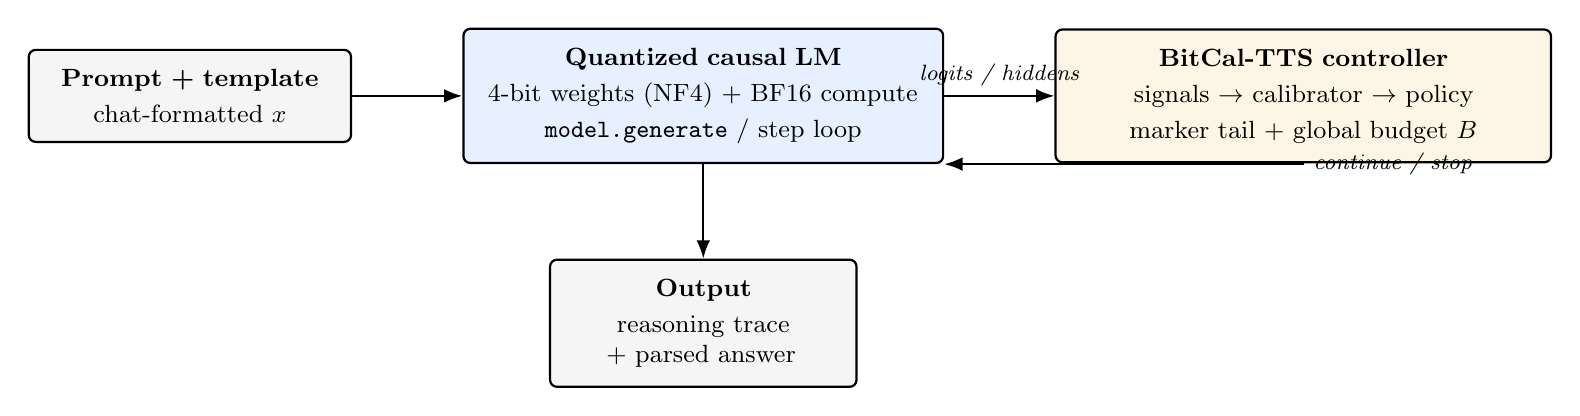
\begin{tikzpicture}[
    font=\small,
    >=Latex,
    box/.style={draw, rounded corners=2.5pt, align=center, inner sep=7pt, thick},
    lbl/.style={font=\footnotesize\itshape}
  ]
    \definecolor{lmfill}{RGB}{230,240,255}
    \definecolor{ctlfill}{RGB}{255,245,230}
    \definecolor{iofill}{RGB}{245,245,245}

    \node[box, fill=iofill, text width=3.6cm] (in) {\textbf{Prompt + template}\\[2pt]{\lbl chat-formatted $x$}};
    \node[box, fill=lmfill, text width=5.6cm, right=14mm of in] (lm) {\textbf{Quantized causal LM}\\[2pt]{\lbl 4-bit weights (NF4) + BF16 compute}\\[2pt]{\lbl \texttt{model.generate} / step loop}};
    \node[box, fill=ctlfill, text width=5.8cm, right=14mm of lm] (ctl) {\textbf{BitCal-TTS controller}\\[2pt]{\lbl signals $\rightarrow$ calibrator $\rightarrow$ policy}\\[2pt]{\lbl marker tail + global budget $B$}};
    \node[box, fill=iofill, text width=3.4cm, below=12mm of lm] (out) {\textbf{Output}\\[2pt]{\lbl reasoning trace + parsed answer}};

    \draw[->, thick] (in) -- (lm);
    \draw[->, thick] (lm) -- node[above, lbl] {logits / hiddens} (ctl);
    \draw[->, thick] (ctl) |- node[near start, right, lbl] {continue / stop} (lm.south east);
    \draw[->, thick] (lm) -- (out);
  \end{tikzpicture}}
  \caption{\textbf{(a) System context.} A frozen quantized backbone exposes logits and last-layer hidden states to a sidecar controller that governs how many tokens are produced under cap $B$.}
  \label{fig:arch-stack}
  \end{subfigure}

  \vspace{4mm}

  \begin{subfigure}{\linewidth}
  \centering
  \resizebox{0.98\linewidth}{!}{%
  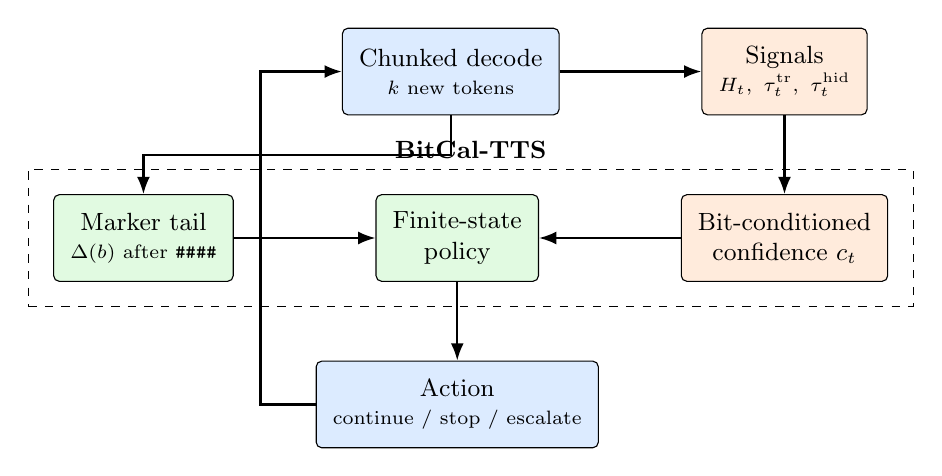
\begin{tikzpicture}[
    font=\small,
    >=Latex,
    node distance=6mm and 8mm,
    box/.style={draw, rounded corners=2pt, align=center, inner sep=6pt, minimum height=11mm},
    flow/.style={thick, -{Latex[length=2.2mm]}}
  ]
    \definecolor{stepc}{RGB}{220,235,255}
    \definecolor{sigc}{RGB}{255,235,220}
    \definecolor{polc}{RGB}{225,250,225}

    \node[box, fill=stepc] (gen) {Chunked decode\\[-1pt]{\scriptsize $k$ new tokens}};
    \node[box, fill=sigc, right=18mm of gen] (sig) {Signals\\[-1pt]{\scriptsize $H_t,\ \tau^{\mathrm{tr}}_t,\ \tau^{\mathrm{hid}}_t$}};
    \node[box, fill=sigc, below=10mm of sig] (cal) {Bit-conditioned\\confidence $c_t$};
    \node[box, fill=polc, left=18mm of cal] (pol) {Finite-state\\policy};
    \node[box, fill=polc, left=18mm of pol] (mar) {Marker tail\\[-1pt]{\scriptsize $\Delta(b)$ after \texttt{\#\#\#\#}}};
    \node[box, fill=stepc, below=10mm of pol] (act) {Action\\[-1pt]{\scriptsize continue / stop / escalate}};

    \draw[flow] (gen) -- (sig);
    \draw[flow] (sig) -- (cal);
    \draw[flow] (cal) -- (pol);
    \draw[flow] (gen.south) -- ++(0,-5mm) -| (mar.north);
    \draw[flow] (mar) -- (pol);
    \draw[flow] (pol) -- (act);
    \draw[flow] (act.west) -- ++(-7mm,0) |- (gen.west);

    \node[draw, dashed, inner sep=9pt, fit=(cal)(pol)(mar), label=above:{\textbf{BitCal-TTS}}] {};
  \end{tikzpicture}}
  \caption{\textbf{(b) Per-step control flow.} After each chunk, signals feed a calibrator; the policy is evaluated only in the pre-marker phase, whereas delimiter detection routes execution through a bit-conditioned tail window.}
  \label{fig:arch-step}
  \end{subfigure}
  \caption{\textbf{Architecture.} BitCal-TTS is a sidecar controller around standard quantized decoding. The marker-aware tail implements answer confirmation that scales with nominal precision.}
  \label{fig:arch}
\end{figure}

\subsection{Problem setup}
Let $x$ be a prompt and $M_b$ a causal language model served at nominal weight precision $b$ (our experiments use $b{=}4$). Let $B$ be a hard cap on newly generated tokens. Decoding proceeds in steps $t{=}1,2,\ldots$; at each step the engine produces a chunk of $k$ tokens (implementation default $k{=}16$), observes logits and optional hidden states, and appends decoded text to partial output $y_{\le t}$.

We compare three methods:
\begin{itemize}
  \item \textbf{Fixed:} always generate until the budget is exhausted or EOS is returned.
  \item \textbf{Adaptive:} apply the halting machinery of Section~\ref{sec:halting}, but feed the calibrator an \emph{effective} precision of 16 bits (making the confidence scale optimistic relative to true 4-bit serving).
  \item \textbf{BitCal-TTS:} identical machinery, but the calibrator uses the true served bit width $b$, and the post-marker tail uses $\Delta(b)$.
\end{itemize}

\subsection{Online signals}
\label{sec:signals}
Let $\ell_t \in \mathbb{R}^{|\mathcal{V}|}$ denote the final-position logits at the end of step $t$, with vocabulary $\mathcal{V}$. Let $p_t = \mathrm{softmax}(\ell_t)$. We use Shannon entropy in nats,
\begin{equation}
  H_t = -\sum_{v \in \mathcal{V}} p_t(v)\,\log p_t(v).
\end{equation}

\paragraph{Reasoning-trace stability.}
Let $(s_1,\ldots,s_t)$ be the sequence of textual chunks produced so far. Writing $\tilde{s}_i$ for the whitespace-stripped chunk, we define a lightweight stability score in $[0,1]$ as the fraction of consecutive pairs $(\tilde{s}_{i-1}, \tilde{s}_i)$ with both lengths at least eight characters that satisfy $\tilde{s}_{i-1}=\tilde{s}_i$. If fewer than two eligible pairs exist, $\tau^{\mathrm{tr}}_t{:=}1$. This proxy rewards literal repetition across recent chunks, which often correlates with the model having settled on a template or final line.

\paragraph{Hidden-state stability.}
When the backend exposes the last-layer hidden vector $h_t \in \mathbb{R}^d$ at the final position of step $t$, we accumulate normalized vectors $\hat{h}_i = h_i / (\lVert h_i\rVert_2 + \epsilon)$ and set $\tau^{\mathrm{hid}}_t$ to the mean cosine similarity between consecutive pairs $(\hat{h}_{i-1}, \hat{h}_i)$ for available indices. If fewer than two vectors exist, $\tau^{\mathrm{hid}}_t{:=}1$.

\subsection{Bit-conditioned confidence}
\label{sec:calibrator}
We map entropy to a normalized uncertainty $u_t = \mathrm{clip}(H_t / H_{\max}, 0, 1)$ with clip-to-interval $[0,1]$ and default $H_{\max}{=}10$. A raw confidence mixes entropy with the two stability proxies,
\begin{equation}
  c^{\mathrm{raw}}_t = w_e(1-u_t) + w_{\mathrm{tr}}\tau^{\mathrm{tr}}_t + w_{\mathrm{hid}}\tau^{\mathrm{hid}}_t,
  \qquad w_e,w_{\mathrm{tr}},w_{\mathrm{hid}} \ge 0,\ \ w_e+w_{\mathrm{tr}}+w_{\mathrm{hid}}=1.
\end{equation}
Weights are renormalized to sum to one for numerical robustness. A bit-width scaling factor $s(b)$ yields
\begin{equation}
  c_t = \mathrm{clip}\bigl(c^{\mathrm{raw}}_t \cdot s(b),\ 0,\ 1\bigr),
  \qquad
  s(b)=
  \begin{cases}
    0.85, & b\le 4,\\
    1.00, & 4<b\le 8,\\
    1.05, & b>8.
  \end{cases}
\end{equation}
Optionally, a temperature $\gamma{>}0$ sharpens or flattens confidence via $c_t \leftarrow \mathrm{clip}(c_t^{1/\gamma},0,1)$. The adaptive ablation sets the calibrator's effective bit width to 16 (so $s{=}1.05$), while BitCal-TTS uses the true served $b{=}4$ (so $s{=}0.85$).

\subsection{Halting policy and marker-aware tails}
\label{sec:halting}
Before the first appearance of the GSM8K delimiter token \texttt{\#\#\#\#} in $y_{\le t}$, we apply a threshold policy with tunable constants. Let $m$ be a minimum number of generated tokens before any halting is allowed (default $m{=}128$). Let $\theta_H$, $\theta_c$, and $\theta_E$ denote entropy stop, confidence stop, and entropy escalate thresholds (defaults $\theta_H{=}2.0$, $\theta_c{=}0.75$, $\theta_E{=}4.0$). Let $r_t$ be remaining budget. With hyperparameter $m_{\mathrm{buf}}$ (implementation \texttt{min\_budget\_to\_continue}${=}32$), the baseline action is
\begin{equation}
  a_t =
  \begin{cases}
    \texttt{continue}, & |y_{\le t}| < m,\\[2pt]
    \texttt{stop}, & |y_{\le t}| \ge m\ \ \text{and}\ \ r_t < m_{\mathrm{buf}},\\[2pt]
    \texttt{escalate}, & |y_{\le t}| \ge m\ \ \text{and}\ \ H_t \ge \theta_E,\\[2pt]
    \texttt{stop}, & |y_{\le t}| \ge m\ \ \text{and}\ \ H_t \le \theta_H\ \ \text{and}\ \ c_t \ge \theta_c,\\[2pt]
    \texttt{continue}, & \text{otherwise.}
  \end{cases}
\end{equation}
Here $|y_{\le t}|$ counts generated tokens. The \texttt{escalate} action is reserved as a deployment hook (e.g., switch to full precision); in our released harness it terminates the step loop like \texttt{stop}.

\paragraph{Post-marker phase.}
Let $t^\star$ be the total number of generated tokens at the first step where \texttt{\#\#\#\#} appears anywhere in the partial output. Define a bit-conditioned confirmation horizon
\begin{equation}
  \Delta(b)=
  \begin{cases}
    32, & b\le 4,\\
    16, & 4<b\le 8,\\
    0,  & b>8.
  \end{cases}
\end{equation}
For both adaptive and BitCal-TTS, once $t^\star$ is defined and $|y_{\le t}|\ge m$, the entropy policy is \emph{bypassed} until the tail constraint is satisfied: if $|y_{\le t}|-t^\star < \Delta(b_{\mathrm{eff}})$, force \texttt{continue}; otherwise force \texttt{stop}. The effective precision $b_{\mathrm{eff}}$ is 16 for adaptive (so $\Delta{=}0$: the delimiter can trigger immediate termination once $m$ is met) and equals the true $b$ for BitCal-TTS (so $\Delta{=}32$ at 4-bit: the model must produce additional tokens after the first delimiter sighting). This implements a precision-dependent tail that reduces false stops driven by brittle low-bit formatting.

\begin{algorithm}[t]
\caption{Budgeted inference with BitCal-TTS (implementation-aligned sketch)}
\label{alg:bitcal}
\begin{algorithmic}[1]
\REQUIRE prompt $x$, cap $B$, chunk size $k$, thresholds, served bit width $b$
\STATE $y \leftarrow \text{empty string}$,\ \ $t^\star \leftarrow \bot$,\ \ $T \leftarrow 0$
\WHILE{$T < B$ \textbf{and not} finished}
  \STATE generate next chunk of up to $k$ tokens; append to $y$; update $T$
  \IF{\texttt{\#\#\#\#} $\in y$ \textbf{and} $t^\star = \bot$}
    \STATE $t^\star \leftarrow T$
  \ENDIF
  \STATE compute $H_t,\tau^{\mathrm{tr}}_t,\tau^{\mathrm{hid}}_t$; set $c_t$ (Section~\ref{sec:calibrator})
  \IF{$T < m$}
    \STATE \textbf{continue}
  \ELSIF{$t^\star \neq \bot$ \textbf{and} $T - t^\star < \Delta(b)$}
    \STATE \textbf{continue}
  \ELSIF{$t^\star \neq \bot$ \textbf{and} $T - t^\star \ge \Delta(b)$}
    \STATE \textbf{stop}
  \ELSE
    \STATE apply entropy policy (Section~\ref{sec:halting})
  \ENDIF
\ENDWHILE
\end{algorithmic}
\end{algorithm}

\subsection{Complexity and overhead}
Each step pays the cost of one forward pass for $k$ tokens plus $O(|\mathcal{V}|)$ work for entropy and $O(d)$ work for cosine tracking. The controller avoids additional model calls: it consumes tensors already materialized for training-style instrumentation.

\section{Experimental setup}
\paragraph{Models and quantization.}
We evaluate \texttt{Qwen/Qwen2.5-3B-Instruct}, \texttt{-7B-}, and \texttt{-14B-} with 4-bit loading via BitsAndBytes as exposed in Transformers~\cite{transformers,bitsandbytes}. Decoding is greedy (\texttt{do\_sample=False}) for reproducibility.

\paragraph{Task, prompts, and extraction.}
We measure exact-match accuracy on GSM8K~\cite{cobbe2021gsm8k} using the standard final-answer extraction protocol after \texttt{\#\#\#\#}. Prompts follow the instruction-tuned chat template for Qwen2.5; the released configuration mirrors the experiment harness in the code repository.

\paragraph{Metrics.}
We report exact-match accuracy, average consumed tokens per example, token savings relative to the fixed baseline at the same $(\text{model}, B)$, and \emph{premature-stop rate}: generation stopped before consuming the full budget \emph{and} the predicted answer is incorrect.

\paragraph{Hardware.}
Primary headline comparisons mirror the tables collected on a single NVIDIA T4 (16\,GB) in Google Colab, reflecting a common low-cost deployment setting.

\section{Results}

\begin{figure}[t]
  \centering
  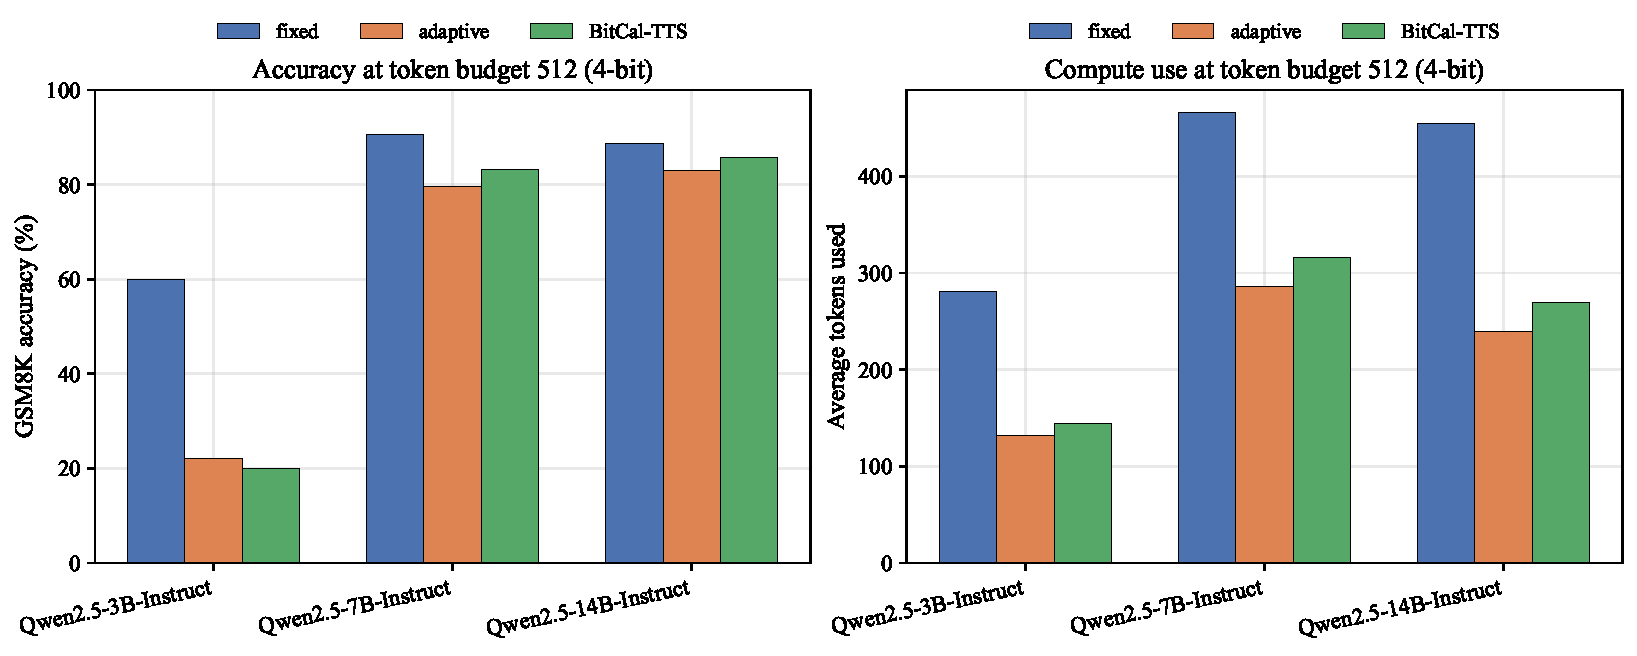
\includegraphics[width=\linewidth]{fig_main_accuracy_tokens.pdf}
  \caption{\textbf{Headline GSM8K comparison at $B{=}512$ (4-bit).} Left: exact-match accuracy. Right: average tokens consumed. BitCal-TTS improves over adaptive on 7B/14B at modest additional cost versus fixed decoding; 3B remains in a regime where halting signals are unreliable relative to task difficulty.}
  \label{fig:main}
\end{figure}

Table~\ref{tab:main} summarizes the primary comparison at $B{=}512$. Figure~\ref{fig:main} visualizes the same aggregates. Figure~\ref{fig:premature} isolates the premature-stop failure mode. Figure~\ref{fig:pareto7b} shows a quality--efficiency scatter for Qwen2.5-7B across budgets using processed summaries, and Figure~\ref{fig:budget7b} traces accuracy and token use as $B$ varies.

\begin{table}[t]
\centering
\caption{GSM8K at token budget 512 (4-bit, headline runs). ``Savings'' is relative to fixed decoding on the same model.}
\label{tab:main}
\begin{tabular}{llrrrr}
\toprule
Model & Method & Acc.\ (\%) & Avg.\ toks & Savings & Prem.\ stop (\%) \\
\midrule
3B  & fixed       & 60.0 & 281 & ---  & 0.0 \\
3B  & adaptive    & 22.0 & 132 & 53.0 & 63.0 \\
3B  & BitCal-TTS  & 20.0 & 144 & 49.0 & 63.0 \\
\midrule
7B  & fixed       & 90.7 & 466 & ---  & 0.0 \\
7B  & adaptive    & 79.6 & 286 & 38.5 & 14.8 \\
7B  & BitCal-TTS  & \textbf{83.3} & 316 & 32.1 & \textbf{11.1} \\
\midrule
14B & fixed       & 88.6 & 455 & ---  & 0.0 \\
14B & adaptive    & 82.9 & 239 & 47.5 & 17.1 \\
14B & BitCal-TTS  & \textbf{85.7} & 269 & 40.8 & \textbf{11.4} \\
\bottomrule
\end{tabular}
\end{table}

\begin{figure}[t]
  \centering
  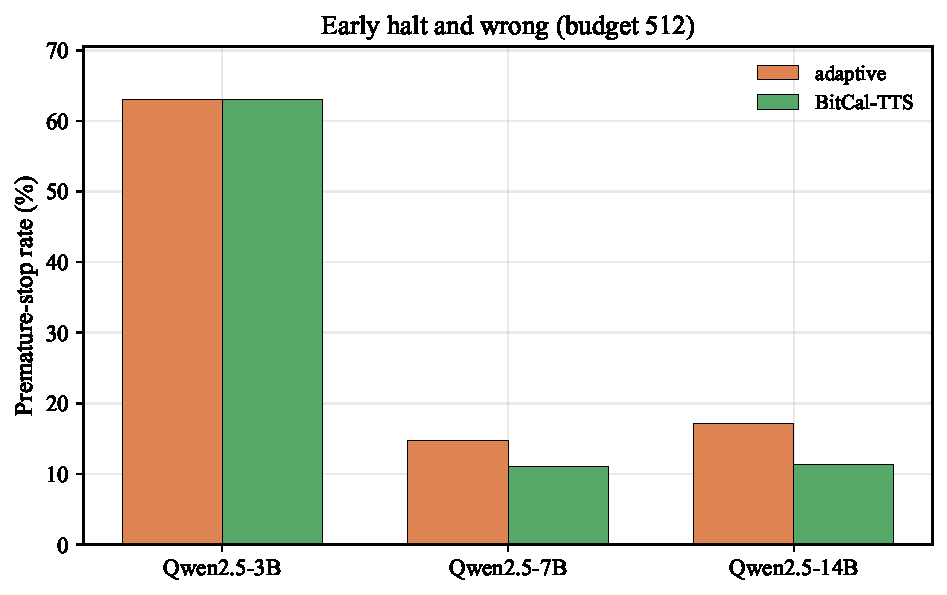
\includegraphics[width=0.75\linewidth]{fig_premature_stop.pdf}
  \caption{\textbf{Premature-stop rate} (halt early \& wrong) at $B{=}512$. BitCal-TTS reduces the failure mode on 7B/14B; 3B remains dominated by weak base reasoning under aggressive early stopping.}
  \label{fig:premature}
\end{figure}

\begin{figure}[t]
  \centering
  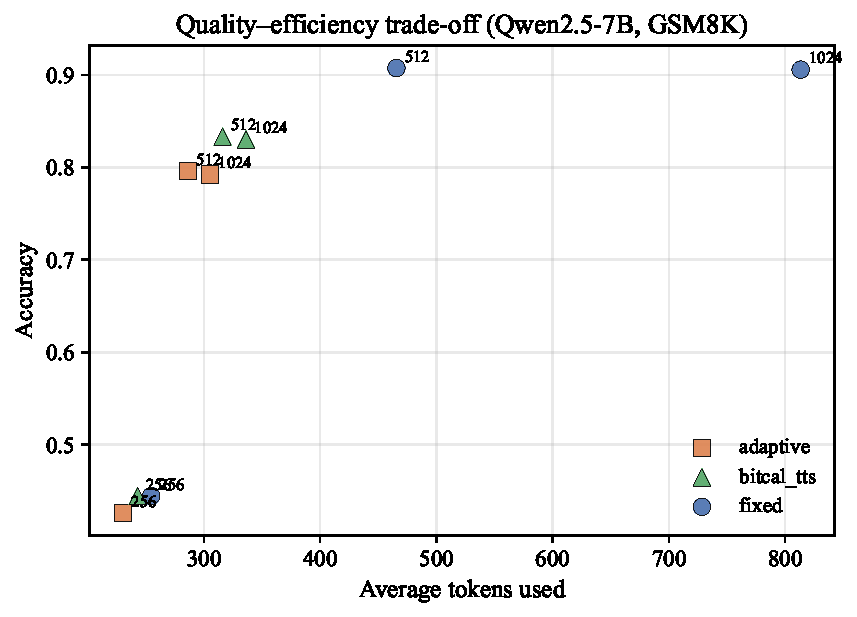
\includegraphics[width=0.72\linewidth]{fig_pareto_7b.pdf}
  \caption{\textbf{Quality--efficiency trade-off (Qwen2.5-7B).} Each point is a method$\times$budget aggregate from \texttt{results/processed/7b/summary.csv}. Budget labels annotate token caps $B$.}
  \label{fig:pareto7b}
\end{figure}

\begin{figure}[t]
  \centering
  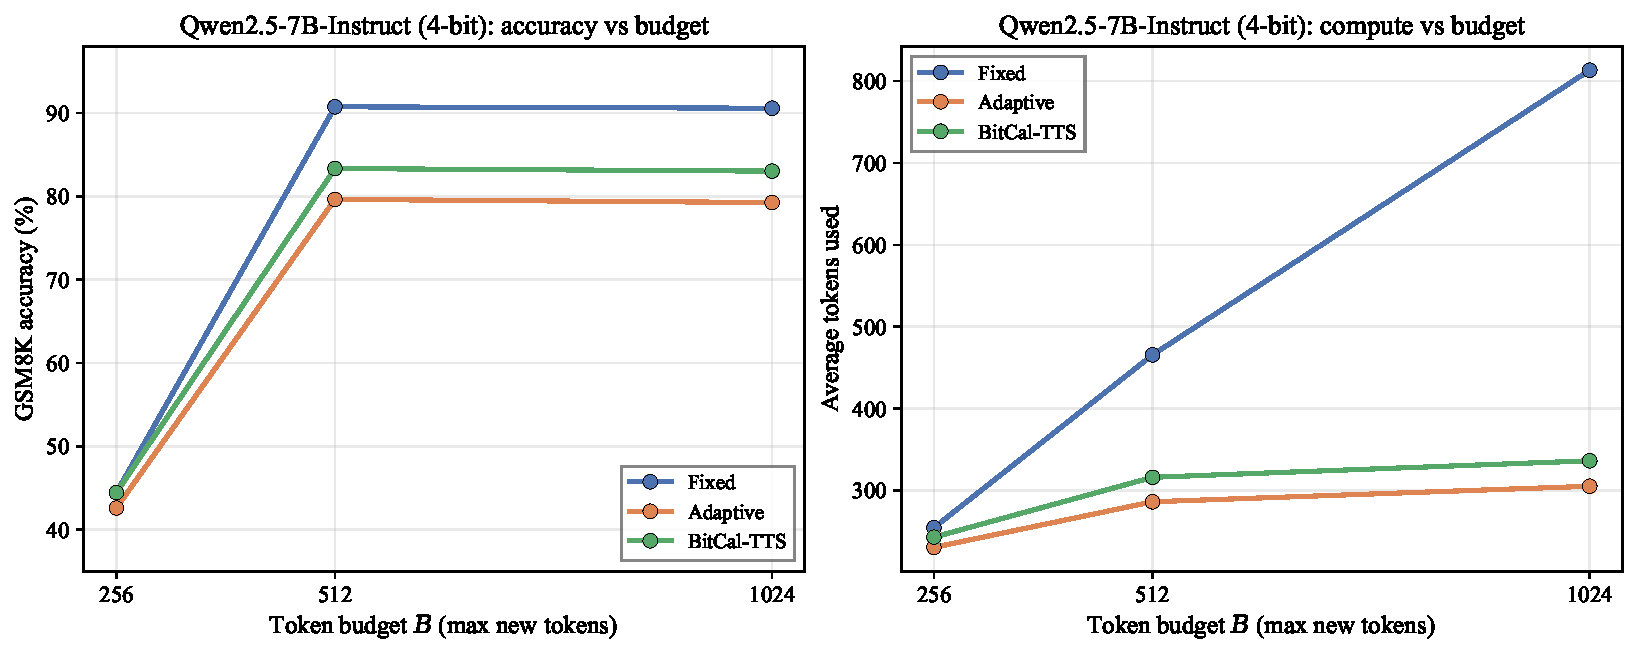
\includegraphics[width=\linewidth]{fig_7b_budget_sweep.pdf}
  \caption{\textbf{Qwen2.5-7B budget sweep (4-bit, processed logs).} Accuracy rises with $B$ for fixed decoding, while adaptive policies plateau earlier. BitCal-TTS tracks closer to fixed accuracy than adaptive at $B{\in}\{512,1024\}$ with substantially lower average token use than fixed.}
  \label{fig:budget7b}
\end{figure}

\subsection{Discussion}
On 7B and 14B, BitCal-TTS sits between adaptive and fixed decoding on token use while improving accuracy over adaptive. The gain is consistent with two mechanisms: (i) conservative confidence scaling at $b{=}4$ reduces entropy-threshold stops that occur while the trace is still unstable, and (ii) the 32-token post-marker tail avoids treating the first delimiter appearance as irrefutable evidence of completion.

At 3B, both adaptive policies collapse: halting signals are unreliable relative to task difficulty, and neither calibration tweak fixes the underlying reasoning gap. BitCal-TTS is a \emph{controller}, not a capacity increase; practitioners should expect diminishing returns when the base model lacks minimal reasoning competence.

\section{Limitations}
Our primary evidence is GSM8K-centric; math reasoning with explicit final markers is a best-case scenario for delimiter-based tails. We do not yet report wall-clock latency or energy, although average tokens are a useful proxy when batching and KV-cache residency dominate. Partial-session runs reduce $N$ for the largest model; Appendix~\ref{app:impl} records the split sizes used in the draft tables. Finally, the policy is intentionally simple; learned calibrators or lightweight verifiers could further improve robustness at the cost of additional engineering.

\section{Conclusion}
We presented BitCal-TTS, a bit-conditioned inference-time controller for quantized reasoning models under a hard token budget. On Qwen2.5-7B/14B in 4-bit, BitCal-TTS reduces premature stops and improves GSM8K accuracy over a non-bit-aware adaptive baseline while preserving large savings versus fixed decoding.

\section*{Acknowledgments}
Experiments were run on Google Colab with NVIDIA T4 GPUs.

\section*{Reproducibility statement}
Code, default hyperparameters, and analysis scripts are available in the accompanying repository. Figures can be regenerated with \texttt{python scripts/paper\_figures.py}. Raw result shards are summarized under \texttt{results/processed/}.

\bibliographystyle{unsrtnat}
\bibliography{references}

\appendix

\section{Notation reference}
\begin{table}[h]
\centering
\begin{tabular}{@{}ll@{}}
\toprule
Symbol & Meaning \\
\midrule
$x$ & Chat-formatted prompt \\
$y_{\le t}$ & Partial generated text after step $t$ \\
$B$ & Hard cap on newly generated tokens \\
$k$ & Tokens generated per controller step \\
$H_t$ & Final-position Shannon entropy at step $t$ (nats) \\
$\tau^{\mathrm{tr}}_t,\tau^{\mathrm{hid}}_t$ & Trace and hidden-state stability scores in $[0,1]$ \\
$c_t$ & Bit-scaled confidence in $[0,1]$ \\
$\Delta(b)$ & Post-marker confirmation tail length \\
$m$ & Minimum tokens before halting \\
\bottomrule
\end{tabular}
\end{table}

\section{Implementation details}
\label{app:impl}
\paragraph{Code and defaults.}
The implementation lives in the \texttt{bitcal\_tts} package with entry points \texttt{scripts/run\_experiment.py} and \texttt{scripts/analyze\_results.py}. Defaults match the released configuration files: step size $k{=}16$; max-entropy normalization $H_{\max}{=}10$; halting thresholds $\theta_H{=}2.0$, $\theta_c{=}0.75$, $\theta_E{=}4.0$; minimum tokens before halting $m{=}128$; minimum remaining budget to allow continuation $m_{\mathrm{buf}}{=}32$; signal weights $(w_e,w_{\mathrm{tr}},w_{\mathrm{hid}}){=}(0.4,0.35,0.25)$; calibrator temperature $\gamma{=}1$.

\paragraph{7B processed aggregates.}
Table~\ref{tab:7blog} lists the Qwen2.5-7B sweep exported from \texttt{results/processed/7b/summary.csv}. Sample sizes reflect the logged shard ($n{=}54$ for $B{\in}\{256,512\}$ and $n{=}53$ for $B{=}1024$).

\begin{table}[h]
\centering
\caption{Qwen2.5-7B across budgets (processed CSV).}
\label{tab:7blog}
\begin{tabular}{lrrrrr}
\toprule
Method & $B$ & $n$ & Acc.\ (\%) & Avg toks & Prem.\ stop (\%) \\
\midrule
fixed      & 256  & 54 & 44.4 & 255 & 0.0 \\
adaptive   & 256  & 54 & 42.6 & 231 & 7.4 \\
BitCal-TTS & 256  & 54 & 44.4 & 243 & 3.7 \\
\midrule
fixed      & 512  & 54 & 90.7 & 466 & 0.0 \\
adaptive   & 512  & 54 & 79.6 & 286 & 14.8 \\
BitCal-TTS & 512  & 54 & 83.3 & 316 & 11.1 \\
\midrule
fixed      & 1024 & 53 & 90.6 & 813 & 0.0 \\
adaptive   & 1024 & 53 & 79.3 & 305 & 18.9 \\
BitCal-TTS & 1024 & 53 & 83.0 & 336 & 15.1 \\
\bottomrule
\end{tabular}
\end{table}

\paragraph{14B partial sweep.}
The draft includes an additional 14B table with $N{\approx}34$--$35$ items per setting due to session limits; we report it explicitly to avoid overstating sample sizes.

\begin{table}[h]
\centering
\caption{Qwen2.5-14B across budgets (partial $N$).}
\begin{tabular}{lrrrrr}
\toprule
Method & $B$ & $N$ & Acc.\ (\%) & Avg toks & Savings \\
\midrule
fixed      & 512  & 35 & 88.6 & 455 & --- \\
adaptive   & 512  & 35 & 82.9 & 239 & 47.5\% \\
BitCal-TTS & 512  & 35 & 85.7 & 269 & 40.8\% \\
fixed      & 1024 & 34 & 91.2 & 859 & --- \\
adaptive   & 1024 & 34 & 82.4 & 235 & 72.6\% \\
BitCal-TTS & 1024 & 34 & 85.3 & 266 & 69.1\% \\
\bottomrule
\end{tabular}
\end{table}

\end{document}
